%-------------------------------------------------------------------------------

% This file is part of Code_Saturne, a general-purpose CFD tool.
%
% Copyright (C) 1998-2014 EDF S.A.
%
% This program is free software; you can redistribute it and/or modify it under
% the terms of the GNU General Public License as published by the Free Software
% Foundation; either version 2 of the License, or (at your option) any later
% version.
%
% This program is distributed in the hope that it will be useful, but WITHOUT
% ANY WARRANTY; without even the implied warranty of MERCHANTABILITY or FITNESS
% FOR A PARTICULAR PURPOSE.  See the GNU General Public License for more
% details.
%
% You should have received a copy of the GNU General Public License along with
% this program; if not, write to the Free Software Foundation, Inc., 51 Franklin
% Street, Fifth Floor, Boston, MA 02110-1301, USA.

%-------------------------------------------------------------------------------

\programme{gradmc}

\vspace{1cm}
%%%%%%%%%%%%%%%%%%%%%%%%%%%%%%%%%%
%%%%%%%%%%%%%%%%%%%%%%%%%%%%%%%%%%
\section*{Fonction}
%%%%%%%%%%%%%%%%%%%%%%%%%%%%%%%%%%
%%%%%%%%%%%%%%%%%%%%%%%%%%%%%%%%%%
Le but de ce sous-programme est de calculer, au centre des cellules, le gradient
d'une fonction scalaire, \'egalement connue au centre des cellules.
Pour obtenir la valeur de toutes les composantes du gradient, une m\'ethode de
minimisation par moindres carr\'es est mise en
\oe uvre~: elle utilise l'estimation d'une composante du gradient aux faces,
obtenue \`a partir des
valeurs de la fonction au centre des cellules voisines. Cette m\'ethode est
activ\'ee lorsque l'indicateur IMRGRA vaut~1 et on l'utilise alors pour le calcul
des gradients de toutes les grandeurs. Elle est beaucoup plus rapide que la m\'ethode
utilis\'ee par d\'efaut (\var{IMRGRA}=0), mais pr\'esente l'inconv\'enient
d'\^etre moins robuste
sur des maillages non orthogonaux, le gradient produit \'etant moins r\'egulier.
% (bien que de m\^eme ordre en espace) J'en sais rien dans l'absolu !.

%%%%%%%%%%%%%%%%%%%%%%%%%%%%%%%%%%
%%%%%%%%%%%%%%%%%%%%%%%%%%%%%%%%%%
\section*{Discr\'etisation}
%%%%%%%%%%%%%%%%%%%%%%%%%%%%%%%%%%
%%%%%%%%%%%%%%%%%%%%%%%%%%%%%%%%%%

\begin{figure}[h]
\parbox{8cm}{%
\centerline{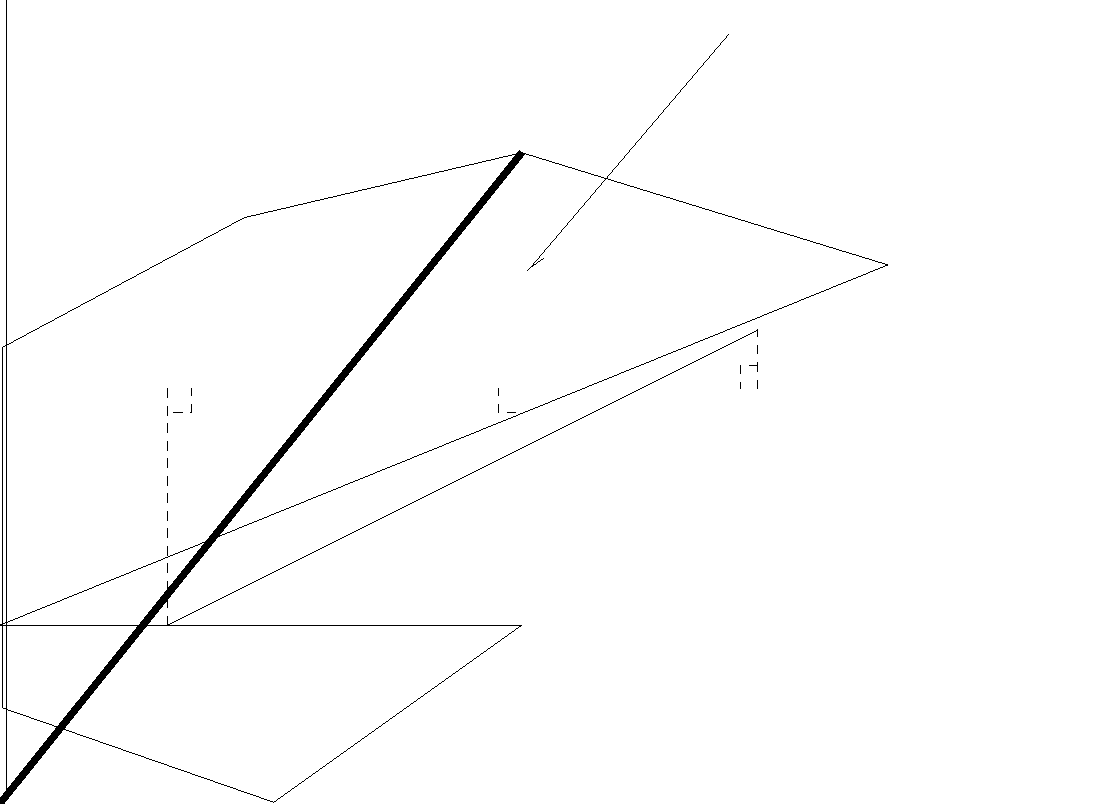
\includegraphics[height=4cm]{facette}}}
\parbox{8cm}{%
\centerline{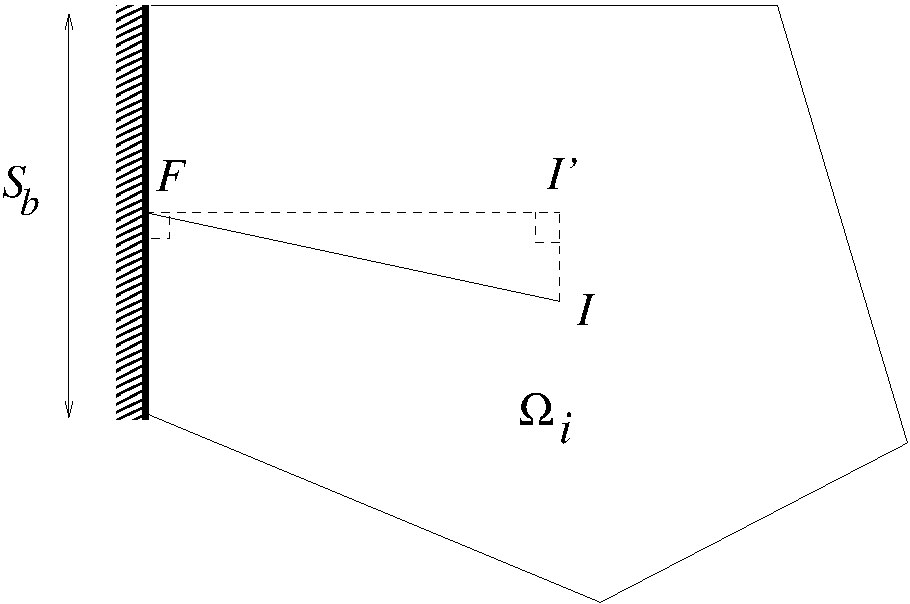
\includegraphics[height=4cm]{facebord}}}
\caption{\label{Base_Gradmc_fig_geom_gradmc}D\'efinition des diff\'erentes entit\'es
g\'eom\'etriques pour les faces internes (gauche) et de bord (droite).}
\end{figure}

On se reportera aux notations de la figure \ref{Base_Gradmc_fig_geom_gradmc}.
On cherche \`a calculer $\vect{G}_{c,i}$, gradient au centre de la cellule $i$ de la
fonction scalaire $P$. Soit  $\vect{G}_{f,ij}\,.\,\vect{d}_{ij}$ une estimation
\`a la face $ij$ (dont les voisins sont les cellules $i$ et $j$)
du gradient projet\'e dans la direction du vecteur $\vect{d}_{ij}$ (\`a pr\'eciser).
De m\^eme, on note
$\vect{G}_{fb,ik}\,.\,\vect{d}_{b,ik}$ une estimation  \`a la face de bord $ik$
($k^{\text{i\`eme}}$ face de bord appuy\'ee sur la cellule $i$) du gradient projet\'e dans
la direction du vecteur $\vect{d}_{b,ik}$ (\`a pr\'eciser).
L'id\'eal serait de pouvoir trouver un vecteur $\vect{G}_{c,i}$ tel que, pour toute
face interne $ij$ ($j\in Vois(i)$) et toute face de bord $ik$
($k\in\gamma_b(i))$, on ait~:
\begin{equation}
\left\{\begin{array}{c}
\vect{G}_{c,i}\,.\,\vect{d}_{ij}=\vect{G}_{f,ij}\,.\,\vect{d}_{ij}\\
\vect{G}_{c,i}\,.\,\vect{d}_{b,ik}=\vect{G}_{f,b,ik}\,.\,\vect{d}_{b,ik}
\end{array}\right.
\end{equation}




Comme il est g\'en\'eralement impossible d'obtenir l'\'egalit\'e, on cherche
\`a minimiser la fonctionnelle~$\mathcal{F}_i$ suivante~:
\begin{equation}\label{Base_Gradmc_eq_fonctionnelle_gradmc}
\mathcal{F}_i(\vect{G}_{c,i},\vect{G}_{c,i})=
\frac{1}{2}\sum\limits_{j\in Vois(i)}\left[
\vect{G}_{c,i}\,.\,\vect{d}_{ij}-\vect{G}_{f,ij}\,.\,\vect{d}_{ij}
\right]^2+
\frac{1}{2}\sum\limits_{k\in \gamma_b(i)}\left[
\vect{G}_{c,i}\,.\,\vect{d}_{b,ik}-\vect{G}_{f,b,ik}\,.\,\vect{d}_{b,ik}
\right]^2
\end{equation}

Pour ce faire, on annule la d\'eriv\'ee de
$\mathcal{F}_i(\vect{G}_{c,i},\vect{G}_{c,i})$
par rapport \`a
chacune des trois composantes ($G_{c,i,x}, G_{c,i,y}, G_{c,i,z}$) du vecteur
inconnu $\vect{G}_{c,i}$ et l'on r\'esout le syst\`eme qui en r\'esulte.

Pour pouvoir inverser le syst\`eme localement et donc \`a faible co\^ut, on
cherche \`a \'eviter les d\'ependances de $\vect{G}_{f,ij}\,.\,\vect{d}_{ij}$ et
de $\vect{G}_{f,b,ik}\,.\,\vect{d}_{b,ik}$ au gradient $\vect{G}_{c,j}$
(gradient pris dans les cellules voisines). Un choix particulier du vecteur
$\vect{d}$ permet d'atteindre ce but~:
\begin{equation}
\vect{d}_{ij} = \frac{\vect{IJ}}{||\vect{IJ}||} \text{\ \ et\ \ } \vect{d}_{b,ik} = \frac{(\vect{I'F})_l}{||\vect{I'F}||}=\vect{n}_{b,ik}
\end{equation}


Ainsi, pour les faces internes, le vecteur $\vect{d}$ est le vecteur norm\'e joignant
le centre des cellules voisines. La quantit\'e
$\vect{G}_{f,ij}\,.\,\vect{d}_{ij}$ est reli\'ee directement aux
valeurs de la variable $P$ prises au centre des cellules, sans faire intervenir
de gradient~:
\begin{equation}
\vect{G}_{f,ij}\,.\,\vect{d}_{ij}=\frac{P_j-P_i}{||\vect{IJ}||}
\end{equation}

Pour les faces de bord, il est possible d'opter pour un choix plus naturel sans pour
autant faire intervenir le gradient des cellules voisines~: on utilise pour
$\vect{d}$ le vecteur
norm\'e orthogonal \`a la face, dirig\'e vers l'ext\'erieur (le gradient le
mieux connu, en particulier au bord, \'etant le gradient normal aux faces).
On a alors~:
\begin{equation}
\vect{G}_{f,b,ik}\,.\,\vect{d}_{b,ik}=\frac{P_{b,ik}-P_{i'}}{||\vect{I'F}||}
\end{equation}

On utilise alors les relations (\ref{Base_Gradmc_eq_val_bord_gradmc}) au bord ($A_{ik}$ et $B_{ik}$
permettent de
repr\'esenter les conditions aux limites impos\'ees, $P_{b,ik}$ en est issue et
repr\'esente la valeur \`a la face de bord)~:
\begin{equation}
\left\{\begin{array}{ll}\label{Base_Gradmc_eq_val_bord_gradmc}
P_{i'}&=P_{i}+\vect{II'}.\vect{G}_{c,i}\\
P_{b,ik}&=A_{ik}+B_{ik}\,P_{i'}=A_{ik}+B_{ik}\,(P_{i}+\vect{II'}.\vect{G}_{c,i})
\end{array}\right.
\end{equation}

On obtient finalement~:
\begin{equation}\label{Base_Gradmc_eq_grad_bord_gradmc}
\vect{G}_{f,b,ik}\,.\,\vect{d}_{b,ik}
=\frac{1}{||\vect{I'F}||}\left[A_{ik}+(B_{ik}-1)\,(P_{i}+\vect{II'}.\vect{G}_{c,i})\right]
\end{equation}

L'\'equation (\ref{Base_Gradmc_eq_grad_bord_gradmc}), qui fait intervenir $\vect{G}_{c,i}$,
doit \^etre utilis\'ee pour modifier
l'expression (\ref{Base_Gradmc_eq_fonctionnelle_gradmc}) de la fonctionnelle avant de prendre sa
diff\'erentielle. Ainsi~:
\begin{equation}\label{Base_Gradmc_eq_fonctionnelle_mod_gradmc}
\begin{array}{ll}
\mathcal{F}_i(\vect{G}_{c,i},\vect{G}_{c,i})=&
\displaystyle\frac{1}{2}\sum\limits_{j\in Vois(i)}\left[
\vect{G}_{c,i}\,.\,\vect{d}_{ij}-\vect{G}_{f,ij}\,.\,\vect{d}_{ij}
\right]^2+\\
&\displaystyle\frac{1}{2}\sum\limits_{k\in \gamma_b(i)}\left[
\vect{G}_{c,i}\,.\,(\vect{d}_{b,ik}-\frac{B_{ik}-1}{||\vect{I'F}||}\,\vect{II'})
-\frac{1}{||\vect{I'F}||}\left(A_{ik}+(B_{ik}-1)\,P_{i}\right)
\right]^2
\end{array}
\end{equation}





On annule alors la d\'eriv\'ee de
$\mathcal{F}_i(\vect{G}_{c,i},\vect{G}_{c,i})$
par rapport \`a
chacune des trois composantes ($G_{c,i,x}, G_{c,i,y}, G_{c,i,z}$) du vecteur
inconnu $\vect{G}_{c,i}$. On
obtient, pour chaque cellule $i$, le syst\`eme $3\times3$ local
(\ref{Base_Gradmc_eq_systeme_matriciel_gradmc})~:
\begin{equation}\label{Base_Gradmc_eq_systeme_matriciel_gradmc}
\underbrace{
\left[\begin{array}{ccc}
\displaystyle
C_{i,x\,x}
& C_{i,x\,y}
& C_{i,x\,z}\\
\displaystyle
C_{i,y\,x}
& C_{i,y\,y}
& C_{i,y\,z}\\
\displaystyle
C_{i,z\,x}
& C_{i,z\,y}
& C_{i,z\,z}
\end{array}\right]
}_{\tens{C}_i}
\underbrace{
\left[\begin{array}{c}
G_{c,i,x} \\ G_{c,i,y} \\ G_{c,i,z}
\end{array}\right]
}_{\vect{G}_{c,i}}
=
\underbrace{
\left[\begin{array}{c}
\displaystyle
T_{i,x}\\
\displaystyle
T_{i,y}\\
\displaystyle
T_{i,z}
\end{array}\right]
}_{\vect{T}_{i}}
\end{equation}

avec


\begin{equation}
\left\{\begin{array}{ll}
C_{i,l\,m} &=\displaystyle
 \sum\limits_{j\in Vois(i)}(\vect{d}_{ij})_{l}(\vect{d}_{ij})_{m}
+\sum\limits_{k\in\gamma_b(i)}\left(\vect{d}_{b,ik}-\frac{B_{ik}-1}{||\vect{I'F}||}\,\vect{II'}\right)_{l}
                              \left(\vect{d}_{b,ik}-\frac{B_{ik}-1}{||\vect{I'F}||}\,\vect{II'}\right)_{m} \\
T_{i,l} &=\displaystyle
 \sum\limits_{j\in Vois(i)}(\vect{G}_{f,ij}\,.\,\vect{d}_{ij})(\vect{d}_{ij})_l
+\sum\limits_{k\in \gamma_b(i)}\frac{1}{||\vect{I'F}||}\left(A_{ik}+(B_{ik}-1)\,P_{i}\right)
                              \left(\vect{d}_{b,ik}-\frac{B_{ik}-1}{||\vect{I'F}||}\,\vect{II'}\right)_l
\end{array}\right.
\end{equation}

On obtient finalement~:
\begin{equation}
\begin{array}{ll}
C_{i,l\,m} &= \displaystyle
\sum\limits_{j\in Vois(i)}\frac{1}{||\vect{IJ}||^2}(\vect{IJ})_l(\vect{IJ})_m
+\sum\limits_{k\in \gamma_b(i)}\left(\vect{n}_{b,ik}+\frac{1-B_{ik}}{||\vect{I'F}||}\,\vect{II'}\right)_{l}
                               \left(\vect{n}_{b,ik}+\frac{1-B_{ik}}{||\vect{I'F}||}\,\vect{II'}\right)_{m}\\
T_{i,l} &=\displaystyle
\sum\limits_{j\in Vois(i)}\left(P_j-P_i\right)\frac{(\vect{IJ})_l}{||\vect{IJ}||^2}
+\sum\limits_{k\in\gamma_b(i)}\frac{1}{||\vect{I'F}||}\left(A_{ik}+(B_{ik}-1)\,P_i\right)
                             \left(\vect{n}_{b,ik}-\frac{B_{ik}-1}{||\vect{I'F}||}\,\vect{II'}\right)_{l}
\end{array}
\end{equation}

%%%%%%%%%%%%%%%%%%%%%%%%%%%%%%%%%%
%%%%%%%%%%%%%%%%%%%%%%%%%%%%%%%%%%
\section*{Mise en \oe uvre}
%%%%%%%%%%%%%%%%%%%%%%%%%%%%%%%%%%
%%%%%%%%%%%%%%%%%%%%%%%%%%%%%%%%%%

La variable dont il faut calculer le gradient est contenue dans le tableau
\var{PVAR}. Les conditions aux limites associ\'ees sont disponibles au travers
des tableaux \var{COEFAP} et \var{COEFBP} qui repr\'esentent respectivement les
grandeurs $A$ et $B$ utilis\'ees ci-dessus. Les trois composantes du gradient
seront contenues, en sortie du sous-programme, dans les tableaux \var{DPDX},
\var{DPDY} et \var{DPDZ}.


\etape{Calcul de la matrice}
Les \var{NCEL} matrices $\tens{C}_{i}$ (matrices $3\times 3$) sont
stock\'ees dans le tableau \var{COCG},
(de dimension $\text{\var{NCELET}}\times 3\times 3$). Ce dernier est initialis\'e \`a z\'ero,
puis son remplissage est r\'ealis\'e dans des boucles sur les faces internes et
les faces de bord. Les matrices $\tens{C}_{i}$ \'etant sym\'etriques, ces boucles ne
servent qu'\`a remplir la partie triangulaire sup\'erieure, le reste \'etant
compl\'et\'e \`a la fin par sym\'etrie.

Pour \'eviter de r\'ealiser plusieurs fois les m\^emes calculs
g\'eom\'etriques, on conserve, en sortie de sous-programme,
dans le  tableau \var{COCG}, l'inverse des \var{NCEL} matrices $\tens{C}_{i}$.
De plus, pour les \var{NCELBR} cellules qui ont au moins une face
de bord, on conserve dans tableau \var{COCGB}, de dimension
$\text{\var{NCELBR}}\times 3\times 3$, la contribution aux matrices $\tens{C}_{i}$
des termes purement g\'eom\'etriques. On pr\'ecise ces points ci-dessous.
Notons donc d\`es \`a pr\'esent qu'il ne faut pas utiliser les tableaux
\var{COCG} et \var{COCGB} par ailleurs comme tableaux de travail.


\hspace*{1cm}{\bf Cellule ne poss\'edant pas de face de bord}\\
Lorsque, pour une cellule, aucune des faces n'est une face de bord du domaine,
l'expression de la matrice $\tens{C}_{i}$ ne fait intervenir que des grandeurs
g\'eom\'etriques et elle reste inchang\'ee tant que le maillage n'est
pas d\'eform\'e. Son inverse n'est donc calcul\'e qu'une seule
fois, au premier appel de \var{GRADMC} avec \var{ICCOCG=1} (l'indicateur
\var{INICOC}, local \`a \var{GRADMC}, est positionn\'e \`a 0
d\`es lors que ces calculs g\'eom\'etriques ont \'et\'e r\'ealis\'es une fois).
Le tableau \var{COCG} est ensuite
r\'eutilis\'e lors des appels ult\'erieurs au sous-programme
\var{GRADMC}.

\hspace*{1cm}{\bf Cellule poss\'edant au moins une face de bord}\\
Lorsque l'ensemble des faces d'une cellule contient au moins une face de bord
du domaine, un terme contributeur aux matrices  $\tens{C}_{i}$ est
sp\'ecifique \`a la variable dont on cherche
\`a calculer le gradient, au travers du coefficient $B_{ik}$
issu des conditions aux limites. Il s'agit de~:

\begin{equation}\label{Base_Gradmc_eq_termes_de_bord_de_C_gradmc}
\sum\limits_{k\in \gamma_b(i)}\left(\vect{n}_{b,ik}+\frac{1-B_{ik}}{||\vect{I'F}||}\,\vect{II'}\right)_{l}
                               \left(\vect{n}_{b,ik}+\frac{1-B_{ik}}{||\vect{I'F}||}\,\vect{II'}\right)_{m}
\end{equation}



Au premier appel r\'ealis\'e avec \var{ICCOCG=1}, on calcule la contribution des faces
internes et on les stocke dans le tableau \var{COCGB}, qui
sera disponible lors des appels ult\'erieurs. En effet, la
contribution des faces internes est de nature purement g\'eom\'etrique et reste
donc inchang\'ee tant que le maillage ne subit pas de d\'eformation. Elle s'\'ecrit~:
\begin{equation}\notag
\displaystyle\sum\limits_{j\in Vois(i)}\frac{1}{||\vect{IJ}||^2}(\vect{IJ})_l(\vect{IJ})_m
\end{equation}
\`A tous les appels r�alis�s avec \var{ICCOCG=1}, les termes
qui d\'ependent des faces de bord (\ref{Base_Gradmc_eq_termes_de_bord_de_C_gradmc}) sont ensuite
calcul\'es et on additionne cette contribution et \var{COCGB} qui contient celle
des faces internes : on obtient ainsi les matrices $\tens{C}_i$ dans le tableau
\var{COCG}. Leur inverse se calcule ind\'ependamment pour chaque
cellule et on le conserve dans \var{COCG} qui sera disponible lors des appels
ult\'erieurs.

Lorsque \var{GRADMC} a \'et\'e appel\'e une fois avec \var{ICCOCG=1},
des calculs peuvent \^etre \'evit\'es en
positionnant l'indicateur \var{ICCOCG} \`a 0 (si
\var{ICCOCG} est positionn\'e \`a 1, tous les calculs relatifs aux cellules
ayant au moins une face de bord sont refaits).

\begin{itemize}
\item [-] Si \var{GRADMC} est utilis\'e pour
calculer le gradient de la m\^eme variable (ou, plus g\'en\'eralement, d'une
variable dont les conditions aux limites conduisent aux m\^emes valeurs du
coefficient $B_{ik}$), les matrices $\tens{C}_{i}$ sont inchang\'ees et leur
inverse est disponible dans \var{COCG} (on positionne \var{ICCOCG} \`a 0 pour
\'eviter de refaire les calculs).
\item [-] Dans le cas contraire, les termes relatifs aux faces de
bord (\ref{Base_Gradmc_eq_termes_de_bord_de_C_gradmc}) sont recalcul\'es et on additionne
cette contribution et \var{COCGB} qui fournit celle
des faces internes : on obtient ainsi les matrices $\tens{C}_{i}$ dans
\var{COCG}. Il reste alors \`a inverser ces matrices.
\end{itemize}

\hspace*{1cm}{\bf Remarque~:}\\
Pour sauvegarder les contributions g\'eom\'etriques dans \var{COCGB}, on a
recours a une boucle portant sur les \var{NCELBR} cellules
dont au moins une face est une face de bord du domaine. Le num\'ero de ces
cellules est donn\'e par \var{IEL = ICELBR(II)} (\var{II} variant de 1 \`a
\var{NCELBR}). Les op\'erations r\'ealis\'ees dans cette
boucle sont du type \var{COCGB(II,1,1) = COCG(IEL,1,1)}. La structure
(injective) de \var{ICELBR} permet de forcer la vectorisation de la boucle.


\etape{Inversion de la matrice}
On calcule les coefficients de la comatrice, puis l'inverse.
Pour des questions de vectorisation, la boucle sur les \var{NCEL} \'el\'ements
est remplac\'ee par une
s\'erie de boucles en vectorisation forc\'ee sur des blocs de \var{NBLOC=1024}
\'el\'ements. Le reliquat ($\var{NCEL}-E(\var{NCEL}/1024)\times 1024$) est
trait\'e apr\`es les boucles.
La matrice inverse est ensuite stock\'ee dans \var{COCG}
(toujours en utilisant sa propri\'et\'e de sym\'etrie).

\etape{Calcul du second membre et r\'esolution}
Le second membre est stock\'e dans \var{BX}, \var{BY} et \var{BZ}. Le gradient
obtenu par r\'esolution des syst\`emes locaux est stock\'e dans \var{DPDX},
\var{DPDY} et \var{DPDZ}.


\etape{Remarque : gradient sans reconstruction} (non consistant sur maillage non
orthogonal)\\
Dans le cas o\`u l'utilisateur souhaite ne pas reconstruire le gradient ({\it
i.e.} ne pas inclure les termes de non orthogonalit\'e au calcul du gradient),
une m\'ethode sp\'ecifique est mise en \oe uvre, qui n'a pas de rapport avec la
m\'ethode de moindres carr\'es pr\'esent\'ee ci-dessus.

Le volume de la cellule $i$ est not\'e $\Omega_i$.
$P_{ij}$ (resp. $P_{b,ik}$) repr\'esente la valeur
estim\'ee de la variable $P$ \`a la
face interne $ij$ (resp. \`a la face de bord $ik$) de vecteur normal associ\'e
$\vect{S}_{ij}$ (resp. $\vect{S}_{b,ik}$). Le gradient est
simplement calcul\'e en utilisant la formule suivante~:
\begin{equation}
\begin{array}{ll}
\vect{G}_{c,i}=
&=\displaystyle\frac{1}{\Omega_i}\left[
\sum\limits_{j\in Vois(i)}P_{ij}\vect{S}_{ij} +
\sum\limits_{k\in\gamma_b(i)}P_{b,ik}\vect{S}_{b,ik}\right]
\end{array}
\end{equation}

Les valeurs aux faces sont obtenues simplement comme suit (avec $\displaystyle\alpha_{ij}=\frac{\overline{FJ'}}{\overline{I'J'}}$)~:
\begin{equation}
\left\{\begin{array}{ll}
P_{ij}
&= \alpha_{ij}P_i+(1-\alpha_{ij})P_j\\
P_{b,ik}
&=A_{ik} +B_{ik}\,P_i
\end{array}\right.
\end{equation}




%%%%%%%%%%%%%%%%%%%%%%%%%%%%%%%%%%
%%%%%%%%%%%%%%%%%%%%%%%%%%%%%%%%%%
\section*{Points \`a traiter}
%%%%%%%%%%%%%%%%%%%%%%%%%%%%%%%%%%
%%%%%%%%%%%%%%%%%%%%%%%%%%%%%%%%%%
\etape{Vectorisation forc\'ee}
Il est peut-\^etre possible de s'affranchir du d\'ecoupage en boucles de 1024 si
les compilateurs sont capables
d'effectuer la vectorisation sans cette aide. On note cependant que ce
d\'ecoupage en boucles de 1024 n'a pas de co\^ut CPU suppl\'ementaire, et que
le co\^ut m\'emoire associ\'e est n\'egligeable.
Le seul inconv\'enient r\'eside dans la relative complexit\'e  de l'\'ecriture.

\etape{Choix du vecteur $d$}
Le choix $\vect{d}_{ij}= \frac{\vect{IJ}}{||\vect{IJ}||}$ permet de calculer
simplement une composante du gradient \`a la face en ne faisant intervenir que
les valeurs de la variable au centre des cellules voisines. Le choix
$\vect{d}_{ij}= \frac{\vect{I'J'}}{||\vect{I'J'}||}$ serait \'egalement
possible, et peut-\^etre meilleur, mais conduirait naturellement \`a faire
intervenir, pour le calcul de la composante du gradient normale aux faces, les
valeurs de la variable aux points $I'$ et $J'$, et donc les valeurs du gradient
dans les cellules voisines. Il en r\'esulterait donc un syst\`eme coupl\'e,
auquel un algorithme it\'eratif (voir \var{GRADRC}) pourrait \^etre appliqu\'e.
L'aspect temps calcul, atout majeur de la m\'ethode actuelle,
s'en ressentirait sans doute.

\etape{Am\'elioration de la m\'ethode}
Cette m\'ethode rencontre des difficult\'es dans le cas de maillages assez ``non
orthogonaux'' (cas de la voiture maill\'e en t\'etra\`edres par exemple). Une
voie d'am\'elioration possible est d'utiliser un support \'etendu (le support est
l'ensemble des cellules utilis\'ees pour calculer le gradient en une cellule
donn\'ee). Un exemple est fourni sur la figure \ref{Base_Gradmc_fig_support_gradmc} ci-dessous~: si la cellule $I$
est la cellule courante, on choisit pour
support les cellules de centre $J$ telles que la droite $(IJ)$ soit la plus
orthogonale possible \`a une face de la cellule $I$.


\begin{figure}[htp]
\centerline{
\includegraphics[height=8cm]{support}}
\caption{\label{Base_Gradmc_fig_support_gradmc}Diff\'erents supports pour le calcul du gradient.}
\end{figure}



